\documentclass[letter, 10pt]{article}
\usepackage[utf8]{inputenc}
%%\usepackage[spanish]{babel}
\usepackage{amsfonts}
\usepackage{amsmath}
\usepackage{graphicx}
\usepackage{url}
% \usepackage{algorithmic}
\usepackage[normalem]{ulem}
\useunder{\uline}{\ul}{}
\usepackage{algorithm}
\usepackage{algpseudocode}
\usepackage[top=3cm,bottom=3cm,left=3.5cm,right=3.5cm,footskip=1.5cm,headheight=1.5cm,headsep=.5cm,textheight=3cm]{geometry}

\begin{document}
\title{Inteligencia Artificial \\ \begin{Large}Informe Final: Problema Radiotherapy Scheduling Problem\end{Large}}
\author{Gabriel Astorga}
\date{\today}
\maketitle


%--------------------No borrar esta secci\'on--------------------------------%
\section*{Evaluaci\'on}

\begin{tabular}{ll}
Mejoras 1ra Entrega (10\%): &  \underline{\hspace{2cm}}\\
C\'odigo Fuente (10\%): &  \underline{\hspace{2cm}}\\
Representaci\'on (15\%):  & \underline{\hspace{2cm}} \\
Descripci\'on del algoritmo (20\%):  & \underline{\hspace{2cm}} \\
Experimentos (10\%):  & \underline{\hspace{2cm}} \\
Resultados (10\%):  & \underline{\hspace{2cm}} \\
Conclusiones (20\%): &  \underline{\hspace{2cm}}\\
Bibliograf\'ia (5\%): & \underline{\hspace{2cm}}\\
 &  \\
\textbf{Nota Final (100)}:   & \underline{\hspace{2cm}}
\end{tabular}
%---------------------------------------------------------------------------%

\begin{abstract}

En este documento se investiga Radiotherapy Scheduling Problem (desde ahora RSP), el cual  tiene como objetivo agendar pacientes con cáncer a sus sesiones de radioterapia, teniendo en cuenta sus prioridades como urgentes, paliativos o radicales, además los tiempos de las máquinas que se utilizarán y los doctores involucrados, todo esto minimizando los tiempos de espera para ser agendados. Además se presenta en detalle la definición del problema, con su respectivo estado del arte, para luego plantear el modelo matemático involucrado en su resolución.
\end{abstract}

\section{Introducci\'on}
El cáncer es uno de los principales causantes de muertes en todo el planeta, de hecho se espera que al no existir una mejora sustancial en el control del cáncer, la cifra de defunciones alcance 13,1 millones de muertes a nivel mundial al año 2030 \cite{nueve}. Uno de los tratamientos para combatir el cáncer focalizado es la radioterapia, el cual utiliza máquinaria como \textbf{LINAC} (acelerador médico lineal, por su siglas en inglés), que sirve para destruir células cancerosas mediante el uso de rayos x. Se clasifica a los pacientes según su progresión del cáncer, a menudo estas corresponden a: \textbf{urgente}, aquellos pacientes que solo son tratados para aliviar el dolor, \textbf{paliativos}, pacientes que siguen un tratamiento sin posibilidad de supervivencia, pero con la esperanza de reducir el dolor a medida que avanza la enfermedad y los pacientes \textbf{radicales}, que tienen una alta expectativa de curación de la enfermedad.


Dado el costo de la máquinaria para tratar el cáncer, sus existencias en hospitales no son bastas con respecto a los pacientes que requieren su uso, además considerando que existen distintos tipos de pacientes que deben ser asignados a ellas y la disponibilidad de los médicos con los que se deben tratar, se convierte en un problema complejo la calendarización manual y rutinaria de los pacientes, considerando los factores de priorización, ocupación y turnos involucrados, por esto se investiga el estado del arte del \textit{Radiotherapy Scheduling Problem}(\textbf{RSP})  y se plantea la forma de automatizar mediante un modelo matemático la asignación de horas o calendarización de pacientes, según los parámetros anteriormente mencionados y profundizados en el presente documento.

\section{Definición del Problema}
El problema a investigar, RSP, es una instancia del conocido problema Job shop\cite{tres} que consiste en encontrar la mejor asignación de recursos a tareas en un determinado tiempo, además tiene otras variantes bastante investigadas, como ESSP (Employee Shift Scheduling Problem), en el cual se busca encontrar la mejor asignación de turnos de trabajos y periodos de descanso a empleados, para un determinado ciclo. El problema tiene como objetivo satisfacer los requisitos de la cantidad de empleados por turno, costo de mano de obra o días libres, minimizando el costo por no cumplir estos objetivos.\cite{doce}

RSP, se basa en la programación de citas al hospital, donde los pacientes deben agendar o reservar distintos tipos de recursos físicos o humanos, para recibir tratamiento o diagnóstico en una serie de tiempo, el problema recae en la minimización de los tiempos de espera de un paciente para ser calendarizados\cite{siete}, además de intentar dar cabida en la agenda a la mayoría de pacientes, considerando su priorización según su categoría, otros enfoques actuales consideran \textit{``la minimización de la desviación general entre los límites de la ventana de tiempo preferida proporcionada por los pacientes y la hora de inicio de sus citas"}\cite{diez}, en general se tiene en cuenta un conjunto de pacientes P sobre un horizonte de calendarización (4 semanas compuesta sólo de días hábiles), discretizado en periodos $\tau$ de tiempo, cuyos pacientes categorizados en  urgentes, paliativos, y radicales son asignables a M máquinas y D doctores. El problema varía dependiendo de los supuestos, consideraciones preferenciales, deterioramiento  del paciente \cite{once} o inclusive el país de estudio; las siguientes restricciones presentadas a continuación son las a tratar:
\begin{itemize}
    \item Solo se puede atender un paciente por máquina y un doctor, cada día.
    \item Para pacientes radicales, paliativos, y urgentes no se debe superar el tiempo de espera de 28, 14, y 2 días, respectivamente. Y tampoco pueden ser menores a 14, 2, y 1 para pacientes radicales, paliativos, y urgentes.
    \item Los pacientes radicales no comienzan su tratamiento los viernes
    \item Los doctores solo pueden atender en los tiempos definidos
    \item La cantidad de sesiones requeridas por cada paciente depende de la gravedad de su
enfermedad. Estas serán 2, 4, y 30 para urgentes, paliativos y radicales, respectivamente.
    \item Los intervalos de tiempo de una máquina o doctor no deben superponerse.
    
\end{itemize}


\section{Estado del Arte}
Entre la década del 60 al 70, se estudia la integración de sistemas computacionales para la gestión de operaciones\cite{uno} que van desde el almacenamiento de la información de un paciente (para no reiterar su registro) hasta la programación de citas para pacientes. Con la evolución de la tecnología y el aumento de la información digitalizada en los centros hospitalarios, los desafíos se volvieron más ambiciosos, por ejemplo en 1986 Kaukiainen, Spring y Wang \cite{dos} proponen un modelo de simulación de un departamento de radiología, con el cual buscaban encontrar los principales factores que influían en el tiempo de tránsito de los pacientes, dónde este dependía principalmente del número de personal y los dispositivos radiográficos, además se justifica la implementación de estos modelos, dada la baja significativa de tiempo en tránsito del paciente pero se deja abierto el problema para mejoras como para los tipos de pacientes que llegan de emergencia. En 2006, Kapamara \cite{tres} en su trabajo para la programación de citas periódicas de radioterapia, clasifica RSP como un complejo problema de job shop scheduling con parámetros especiales, Job shop es un problema altamente estudiado los últimos 40 años, el cual es reconocido por ser NP-difícil \cite{cuatro}, por ende RSP es un problema altamente complejo, que puede ser abordado con heurísticas. 
\\
Este problema es relativamente reciente, y su estudio está vigente al día de hoy, por lo que a continuación se presentan las últimas heurísticas para su resolución.

\subsection{Métodos de resolución}
    \subsubsection{GRASP}
    En 2006, Petrovic \cite{cinco} presenta un estudio con enfoques para resolver scheduling problems relacionado a RSP, aquí categoriza a pacientes por prioridad (Emergencia, urgente o rutina) y tratamiento (radical, paliativo o adyuvante), los cuales tienen un objetivo de tiempo de espera (fecha de vencimiento), además define cuatro enfoques para generalizar métodos ASAP y JIP estudiados anteriormente \cite{seis}.
    \\El \textbf{primero} se basa en predefinir un valor target para definir el primer día para que se empiece a intentar agendar a un paciente (el cuál al final menciona que no es un buen enfoque). El \textbf{segundo} es definir un ``threshold" para la utilización de cada máquina, según la prioridad del paciente. El \textbf{tercero} se define como SCD (``Schedule Creation Day") y toma la información de los enfoques anteriores y se selecciona un día específico en la semana para comenzar a intentar agendar a un paciente. Y el \textbf{cuarto} y último corresponde a MNDA (``Maximum Number of Days in Advance"), dónde se fija una ventana de tiempo para la asignación del primer tratamiento, unificando también la información entregada por los enfoques anteriores.
    \\Finalmente centraliza su estudio en la creación de un algoritmo que usa metaheurísticas, ``Greedy Random Adaptive Search Procedure" (GRASP) el cual consta de dos fases que se repiten durante varias iteraciones, donde la primera corresponde a ordenar pacientes según prioridad y luego se aplica búsqueda local, comparando pacientes al azar que no cumplen el objetivo de tiempo de espera, con pacientes que necesitan el mismo tipo de radiación, situándoles con precedencia en fecha. 
    Los resultados que obtiene son que en el 38\% de los casos logró superar los enfoques constructivos, y el 23\% provocó que el calendario fuera peor que el de algoritmos constructivos. 

\subsubsection{RASON}
    En 2016 M. Riff publica un nuevo enfoque para la resolución de RSP \cite{siete}, en el cuál se propone RASON (``Radiotherapy Scheduling with ON-the-fly priorities"), el cuál también minimiza el tiempo de espera del paciente, pero puede gestionar dinámicamente la prioridad de un paciente según su categoría y tiempo de espera actual. Además se auto-evalúa con datos reales del Instituto de Radioterapia de Santiago, Chile y datos generados sintéticamente. Este algoritmo define los mismos parámetros y restricciones que los mencionados anteriormente \cite{seis}, y supera los algoritmos ASAP y JIP con una significancia estadística del 95\%. Otro aporte adicional de este trabajo es que utiliza búsqueda local, para ser aplicado en RSP del mundo real y tener en cuenta el tiempo de espera actualizado de los pacientes. Este algoritmo se basa en dos fases, la primera utiliza greedy para calendarizar pacientes de la semana actual y luego se realiza búsqueda local para mejorar el calendario (solución inicial), esta búsqueda se basa en hacer uso de tres algoritmos Hill climbing (HC) sucesivos, dónde su función de evaluación corresponde a ``\textit{la suma de los retrasos de todos los pacientes planificados esta semana por el algoritmo greedy o en lista de espera}". El primer HC hace dos movimientos swap, uno movimiento es entre un paciente recién agendado y uno en lista de espera y otro selecciona un paciente en lista de espera y lo calendariza si es posible. El segundo HC intenta cambiar dos pacientes ya calendarizados que partirán su tratamiento la semana actual pero en dos días diferentes. Por último el tercer HC intenta mitigar los espacios vacíos que dejando los dos anteriores, adelantando los tratamientos en la semana. Como se menciona al principio RASON es superior que los algoritmos presentados por Petrovic, pudiendo agendar mejor y más pacientes, aún así no se compara ni se presenta el tiempo de cómputo de estos pero si su efectividad.
    \subsection{Algoritmos en línea}
    En 2019 se publica \textit{''Health Care Systems Engineering"} por Bélanger et al. \cite{trece} el cual reúne distintos problemas que la literatura intenta resolver en el área de la salud y entre ellos está el RSP, dónde se compara los enfoques y resultados de distintos autores, incluidos los dos anteriores, y bajo la misma categorización de pacientes y los días que necesitan tratamiento, intenta dar una nueva mejora a los algoritmos de calendarización en línea, dada las características del problema. “Calendarización en línea” refiere a que los pacientes se actualizan con el tiempo, por lo que las citas deben ser calendarizadas sin saber la demanda futura. Los autores comparan 5 algoritmos de la literatura mejorados y/o creados por ellos, los mejorados son \textbf{SASAP} (``smart ASAP"), \textbf{SJIT} (``smart JIT) y los otros tres  se crean a partir de observación de patrones en las soluciones de modelos de programación lineal entera, pero para instancias pequeñas, que se denomina ``fountain effect", que consiste en anidar ``ganchos" \footnote{formas que se producen al agendar pacientes en distintos días en slots de tiempos consecutivos, dejando un espacio vacío en la ``curvatura del gancho" que no se puede agendar a nadie por falta de continuidad, para visualizar ver \cite{trece} pág. 253} del mismo tipo (derecho o izquierdo) en los dos lados del turno (desde el principio hacia adelante o desde el final hacia atrás, respectivamente), estos algoritmos en línea son, \textbf{FOS} (fountain on shift), cumpliendo lo antes mencionado, y para las máquinas con dos turnos por día se tiene \textbf{FOM} (fountain on machine), y como se observa que anidar pequeños ganchos con dos largos produce desperdicios de ranuras en el calendario, se propone \textbf{SFOM} (selective fountain on machine) que asigna previamente una categoría a cada turno en proporción a la demanda esperada y explota el fountain effect en el turno seleccionado. Los resultados para FOS y SFOM son bastante buenos, donde FOS logra disminuir los tiempos de espera con respecto a SASAP entre 3 a 7 días con un 6-11\% más de pacientes tratados dentro de la fecha de vencimiento. SFOM obtiene los mejores resultados, casi todos los días logra agendar 4 pacientes más y todos ellos son tratados con tiempos de espera muy bajos, siendo estos menores en 4-20 días que ASAP y 26-40 días menos que SJIT, y considerando el escenario de evaluación sobrecargado de pacientes SFOM es capaz de tratar dentro de la fecha de vencimiento a todos los pacientes urgentes.


\section{Modelo Matemático}
El modelo que se presenta en este trabajo es propuesto por Petrovic et al. en 2011 \cite{ocho}, cuyo espacio de búsqueda, depende de los N pacientes por el tamaño del calendario o agenda, que corresponde a O operaciones en el día por D días que dure la planificación (no se consideran M máquinas, por el modelo y por que no se hace diferencia entre usar uno u otro LINAC), lo que correspondería a un espacio $E.B= N \cdot O \cdot D$. El modelo descrito se presenta a continuación.

\subsection{Parámetros}

\begin{tabular}{llr}
\hline
\multicolumn{2}{c}{\textbf{Tabla 1.} Parámetros RSP} \\
\cline{1-2}
\hline
\textbf{Parámetro}    & \textbf{Descripción} \\
\cline{1-2}\hline
N &    Número de pacientes recibidos dentro de un horizonte de calendarización.
\\\hline
j &    paciente, j = 1, 2 ,... , N 
\\\hline
M &    Conjunto de máquinas e instalaciones.
\\\hline
k &    Máquina o instalación, k e M
\\\hline
H &    Número total de doctores
\\\hline
h &    Doctor, h = 1, 2, ... , H
\\\hline
$h_{j}$ &    Doctor asignado al paciente j
\\\hline
$H_{h}$ &    Disponibilidad de un doctor h en la lista de rotación del hospital.  
\\\hline
(i, j, k) &    Operación i de un paciente j sobre una máquina o instalación k
\\\hline
($i^{f}$, j, k) &    La primera fracción de tratamiento $i^{f}$ del paciente j en la máquina k     
\\\hline
$S_{(i,j,k)}$ &    Día en que la operación i para el paciente j en la máquina o instalación k parte    
\\\hline
$\tau_{(i,j,k)}$ &    Tiempo de procesamiento de la operación i del paciente j en la máquina o instalación k   
\\\hline
$C_{(i,j,k)}$ &    Tiempo de finalización de la operación i del paciente j en la máquina o \\& instalación k, $C_{(i,j,k)} = S_{(i,j,k)} + \tau_{(i,j,k)}$   
\\\hline
$r_{j}$ &          Momento en el que se toma la decisión de tratar con radioterapia al paciente j.
\\\hline

$d_{j}$ &          Objetivo de tiempo de espera para la primera fracción de tratamiento del paciente
\\& j; Se denominará ``fecha de vencimiento" (``due date")  
\\\hline

E &          Categoría paciente urgente    
\\\hline
P &          Categoría paciente paliativo
\\\hline
R &          Categoría paciente Radical   
\\\hline
$C_{j}$ &    Categoría del paciente j  
\\\hline
$W_{j}$ &    Peso dado al paciente j basado en su categoría    
\\\hline

RTM(k) &     Calendarización existente de una máquina o instalación k, RTM(k) = \{[$s_{(i,j,k)}$, $C_{(i,j,k)}$] $\mid$
\\& tiempos de inicio y finalización de todas las operaciones de todos los pacientes programados 
\\& en la máquina o intalación k\} 
\\\hline

RTD(h) &     Calendarización existente de doctores, RTD(h) = \{[$s_{(i,j,h)}$, $c_{(i,j,h)}$] $\mid$ conjunto de tiempos 
\\&de inicio y finalización de todas las operaciones de todos los pacientes programados al doctor h\}

\\\hline
$F_{j}$ &            Tiempo de flujo desde la unidad de planificación a la de tratamiento del paciente j \\&  (Tiempo de espera del paciente j), 
$F_{j} = S_{(i_{f}, j, k)} - r_{j}$
\\\hline
$\bar{F}$  &         Tiempo promedio de flujo de N pacientes atendidos dentro de un horizonte de calendarización
\\& (tiempo promedio de espera),  $\bar{F} = \frac{1}{N}\sum_{j=1}^{N}{F_{j}}$
\\\hline
$\bar{F}_{w}$ &     Tiempo de flujo promedio de N pacientes atendidos dentro de un horizonte de calendarización
\\& $\bar{F}_{w} = \frac{1}{N}\sum_{j=1}^{N}{w_{j}F_{j}}$
\\\hline
\hline
\end{tabular}

\subsection{Función Objetivo}
MIN $\bar{F}= \frac{1}{N}\sum_{j=1}^{N}{F_{j}}$
\subsection{Restricciones}
Restricción de capacidad de la máquina o instalación k\\
\begin{itemize}
    \item  RTM(k) = \{ [$s_{(i,j,k)}$, $C_{(i,j,k)}$] $\mid$ los intervalos de tiempos [$s_{(i,j,k)}$, $C_{(i,j,k)}$] no se superpongan para todo i,j \}
\end{itemize}
Restricción de capacidad del doctor h 
\begin{itemize}
    \item   RTD(h) = \{[$s_{(i,j,h)}$, $c_{(i,j,h)}$] $\mid$ los intervalos de tiempos [$s_{(i,j,h)}$, $C_{(i,j,h)}$] no se superpongan para todo i,j \}
\end{itemize}
Tiempos de retardo de operaciones consecutivas i e (i+1) del paciente j para cualquier máquina o instalación k y k', donde k, k' $\in$ M

\begin{itemize}
    \item $S_{(i,j,k)} - S_{(i+1, j, k')}+ \tau_{i, j, k)} \leq 0$, where $k \neq k'$
    \item $S_{(i,j,k)} \geq 0$
    \item $\tau_{(i,j,k)} \geq 0$
    \item k = 1,2,...,$\lvert M \rvert$
    \item j = 1,2,..., N
    \item h = 1,2,...,H
\end{itemize}

\subsection{Supuestos}
El modelo formula los siguientes supuestos
\begin{enumerate}
\item Las instalaciones de radioterapia siguen estrictamente una semana laboral de cinco días, es decir, de lunes a viernes.
\item Los pacientes radicales no comienzan sus tratamientos los viernes.
\item Solo se puede dar servicio a un paciente en una máquina a la vez.
\item No se permite la preferencia, es decir, una vez que se inicia la operación en una máquina o instalación, no se puede interrumpir.
\item Todas las operaciones para los pacientes se conocen de antemano y están listas para comenzar a procesar al comienzo del horizonte de tiempo considerado.
\item Los tiempos de procesamiento de todas las operaciones y las restricciones de precedencia son deterministas y se conocen de antemano.
\item El tiempo de procesamiento de cada operación no depende de la secuencia en la que se procesan las operaciones.
\item Se conocen los tiempos en que los pacientes están disponibles para iniciar los procesos de radioterapia.
\item Los pacientes se clasifican en tres categorías: radicales, paliativos y de emergencia con objetivos de tiempo de espera; fechas de vencimiento de 28, 14 y 2 días, respectivamente.
\item Los tiempos de preparación de las máquinas o instalaciones y los tiempos de transferencia entre máquinas o instalaciones se consideran insignificantes en comparación con los tiempos de procesamiento.
\item No hay reciclados en máquinas e instalaciones, excepto en linacs; un paciente visita una máquina o instalación una vez, lo que significa que se debe realizar una sola operación en una máquina o instalación para cada paciente.
\item Las máquinas e instalaciones están siempre disponibles durante el turno. No se consideran las operaciones de avería y mantenimiento. El poder del hombre de habilidad uniforme está disponible.
\item Los médicos están disponibles en una rotación del hospital.
\item Una vez que comienza una entrega de fracciones, debe continuarse todos los días excepto los fines de semana y feriados hasta que se complete
\end{enumerate}




\section{Representación}
Para efectos de este trabajo se realizará la implementación de un algoritmo de búsqueda local que se base en parte de Tabú Search como algoritmo reparador, y Greedy para construir su solución inicial, con el objetivo de disminuir los tiempos de espera de los pacientes. Además, se aborda la capacidad de mejorar la solución, basándose en la asignación de las mismas máquinas y mismos doctores para un paciente.

Como representación se utilizan dos matrices que representan la asignación calendarizada paciente-doctor o paciente-máquina, dónde las filas representan a los pacientes, las columnas el bloque/día correspondiente y el valor de las casillas son el doctor/máquina asignado(a).
Para el siguiente ejemplo se tiene un extracto de la matriz, dónde se representa la asignación del doctor 1 al paciente j en el bloque 1 del día i:



\begin{table}[ht]
\centering
\begin{tabular}{l|lllll|l|}
\cline{2-7}
 &  &  & Día i &  &  & ... \\ \cline{2-7} 
& \multicolumn{1}{l|}{B1}  & \multicolumn{1}{l|}{b2}  &\multicolumn{1}{l|}{...} & \multicolumn{1}{l|}{Bn-1} & Bn  & ... \\ \hline
\multicolumn{1}{|l|}{paciente j} & \multicolumn{1}{l|}{1}   & \multicolumn{1}{l|}{0}   & \multicolumn{1}{l|}{0}   & \multicolumn{1}{l|}{0}    & 0   & ... \\ \hline
\multicolumn{1}{|l|}{...}        & \multicolumn{1}{l|}{...} & \multicolumn{1}{l|}{...} & \multicolumn{1}{l|}{...} & \multicolumn{1}{l|}{...}  & ... & ... \\ \hline
\end{tabular}
\caption{Representación asignación paciente-doctor.}
\label{table:ta}
\end{table}

Además se utilizan vectores para paciente y máquinas, con largo igual a la cantidad respectiva de cada uno, y una matriz para los doctores, con tamaño igual a la cantidad de doctores por los días de una semana hábil, todo esto con la finalidad de contabilizar la cantidad de sesiones que le restan a cada paciente, los días disponibles de cada doctor y la disponibilidad de las máquinas, dado que la representación de las máquinas solo es una lista con el número de la máquina, no se explicita, en cambio las representaciones de paciente y doctor, necesitan un entendimiento más a fondo. Las sesiones de un paciente se representan del siguiente modo.

\begin{table}[h]
\centering
\begin{tabular}{|c|c|c|c|c|c|c|}
\hline
SesiónPaciente1 & SesiónPaciente2 & ... & SesiónPaciente\_i & ... & SesiónPaciente\_n \\ \hline
\end{tabular}
\caption{Representación sesiones paciente.}
\label{table:pa}
\end{table}

Dónde la casilla i hace referencia al paciente i y corresponde a las sesiones que lleva en total.
En el caso de los doctores se tiene una matriz, dónde las columnas corresponden a los días  y las filas a los doctores, indicando su disponibilidad de turno\footnote{Estos valores corresponden a 1:mañana, 2: tarde, 3:mañana y tarde}, y su estructura tiene la siguiente forma.

\begin{table}[ht]
\centering
\begin{tabular}{l|l|l|l|l|l|}
\cline{2-6}
                                & Día\_1 & Día\_2 & Día\_3 & Día\_4 & Día\_5 \\ \hline
\multicolumn{1}{|l|}{doctor\_1} & 1      & 0      & 2      & 3      & 0      \\ \hline
\multicolumn{1}{|l|}{...}       & ..     & ..     & ...    & ...    & ...    \\ \hline
\multicolumn{1}{|l|}{doctor\_h} & 1      & 1      & 2      & 2      & 3      \\ \hline
\multicolumn{1}{|l|}{...}       & ...    & ...    & ...    & ...    & ...    \\ \hline
\multicolumn{1}{|l|}{doctor\_n} & 3      & 3      & 0      & 0      & 1      \\ \hline
\end{tabular}
\caption{Representación disponibilidades doctor h para día hábil.}
\label{table:pab}
\end{table}

\newpage
\section{Descripción del algoritmo}
El algoritmo desarrollado en este trabajo se compone de dos fases, la primera se basa en la utilización de un algoritmo constructivo llamado ``\textit{Greedy algorithm}" y la segunda fase hace uso de un algoritmo reparador, ``\textit{Tabu Search}", esto para mejorar la solución entregada por el primer algoritmo.A continuación se definen las funciones asociadas a cada algoritmo y el movimiento realizado por el algoritmo reparador.

\subsection{Primera fase}
La primera fase utiliza un algoritmo greedy, el cuál parte construyendo su solución con los pacientes urgentes, luego con los paliativos y por último con los radicales, como la característica intrínseca de greedy es tomar lo mejor para la solución actual, la función miope se basa en asignar al paciente el primer doctor/máquina disponible.

\begin{algorithm}[H]
  \caption{$Greedy Algorithm$}\label{greedy}
  \begin{algorithmic}[1]
    \Procedure{Greedy}{$Cola Pacientes, maquinas, schedule_{doctores}$}
    \For{\texttt{day < 20}}
        \State $Q_{paciente}\gets Queue\_sort(Pacientes, day)$
        \For{\texttt{bloque < 16}}
            \State $ Q_{Maq}\gets Queue\_sort(maquinas)$
            \State $ Q_{doctor}\gets Queue\_sort(schedule_{doctores}[dia\_actual(day)], bloque)$
            
            \While{\texttt{not empty} $Q_{doctor}$ \texttt{and not empty} $Q_{Maq}$ \texttt{and not empty} $Q_{paciente}$}
            
                \State $ paciente_{asigned}\gets get(Q_{paciente})$
                \State $ doctor_{asigned}\gets get(Q_{doctor})$
                \State $ machine_{asigned}\gets get(Q_{machine})$ 

                \State $ schedule\_p\_doctor[paciente_{asigned}][day*bloques + bloque] \gets doctor_{asigned}$
                \State $ schedule\_p\_machine[paciente_{asigned}][day*bloques + bloque]\gets machine_{asigned}$
                \If {(Pacientes = 0)}
                       \State break\;
                \EndIf
                
            \EndWhile
        \EndFor
    \EndFor
      \State \textbf{return} \texttt{schedule\_p\_doctor, schedule\_p\_machine}
    \EndProcedure
  \end{algorithmic}
\end{algorithm}

La idea principal del \textit{Algoritmo 1} es realizar una asignación priorizando la clasificación del paciente, la disponibilidad del personal y los recursos, para esto se itera todo el calendario de 20 días, cada uno compuesto de 16 bloques, dónde cada día se construye una cola de prioridad de los pacientes a ser atendidos, en ella se considera las restricciones asociadas al paciente,\footnote{Como que los radicales no pueden ser atendidos antes de los 14 días o que no empiezan su tratamiento los viernes.} si terminaron sus sesiones y por ende no necesitan ser agendados, o el caso contrario en el que ya empezaron su primera sesión y por ende deben ser agendados para que no tengan interrupciones en su tratamiento. Otra cola utilizada es la de máquinas, dónde se encolan todas las máquinas disponibles el día y bloque correspondiente, también se utiliza la cola de doctores, la cual tiene los doctores disponibles según día y bloque, correspondiente a su horario de atención. 

\subsection{Segunda fase}
    Esta fase se basa en reparar la solución entregada anteriormente, usando la implementación del algoritmo de búsqueda local \textit{Tabu Search}. Dado que la primera parte entrega los pacientes agendados lo más a la izquierda posible, no se consideraran los tiempos de espera, dado que esto significaría, adelantar pacientes de otras categorías lo cuál va en contra de las restricciones y solo produciría soluciones infactibles, por lo que se propone definir una medida de calidad en base a la ``\textit{satisfacción final}" del paciente, esto se basa en el supuesto de que un paciente preferiría mantener el doctor con el que se trata y posiblemente acostumbrarse a utilizar una máquina ``\textit{personal}". Mas en detalle, para mejorar la solución se maximiza las máquinas y doctores asociadas al mismo paciente, lo que implica que, si un paciente empezó con el doctor d y la máquina m, lo ideal sería que terminase su tratamiento con los mismos o sin sufrir muchos cambios.

\begin{algorithm}[H]
  \caption{$ Tabu Search$}\label{TS}
  \begin{algorithmic}[1]
    \Procedure{Tabu}{$solution_{doctor}, solution_{machine}, max\_size, U,P,R, stop\_criterion$}
    \State $Tabu_{list} \gets initialize$
    \State $  S\_best\_d \gets solution_{doctor}$ 
    \State $  S\_best\_m \gets solution_{machine}$ 
    \While{$stop\_criterion$}
    
        \State $ S\_v\_d, S\_v\_m \gets best\_N(solution_{doctor}, solution_{machine}, Tabu_{list}, U,P,R);$
        \State $ doctor_{asigned}\gets Q_{doctor}$
        \State $ machine_{asigned}\gets Q_{machine}$

        \State $ update\_tabu\_list(forbidden\_movement)\;$
        \If {$f_{ev}(S\_v\_d, S\_v\_m, N_{pacientes}) \geq f_{ev}(S\_best\_d, S\_best\_m, N_{pacientes})$}
            \State $ S\_best\_d \gets S\_v\_d$ 
            \State $ S\_best\_m \gets S\_v\_m$ 
        \EndIf
        
    \EndWhile
            
      \State \textbf{return} \texttt{S\_best\_d, S\_best\_m}
    \EndProcedure
  \end{algorithmic}
\end{algorithm}

El algoritmo de \textit{Tabu search} recibe la solución construida en el paso anterior por \textit{Greedy}, dónde se evalúa el calendario de las máquinas y de los doctores, lo interesante a analizar en este algoritmo es su función de evaluación y el movimiento para generar los vecindarios.
\subsubsection{Función de evaluación}
La función de evaluación dicta la calidad de la solución en base a contabilizar cuantas veces se le asigna el mismo doctor a un paciente, de la misma forma se contabilizan las máquinas asociadas, y se suman considerando un peso para la asignación de doctores y máquinas, este peso es un número mayor para los doctores, para priorizar la asignación de mismos doctores antes que mismas máquinas.

\begin{equation}\label{eq:1}
    0.7*\dfrac{\sum{X_{jh} + X_{jh'}}}{2} + 0.3*\dfrac{\sum{X_{ik} + X_{ik'}}}{2}, \forall h=h', k=k'
\end{equation}
h corresponde a los doctores y k a las máquinas.

\subsubsection{Movimiento}
El movimiento realizado se basa en hacer swap entre pacientes pero para un día en específico, y solo entre pacientes pertenecientes a la misma categoría\footnote{e.g. radicales intercambian horarios con radicales, paliativos con paliativos y urgentes con urgentes}, esto último para realizar movimientos factibles con respecto a la asignación del paciente en el horiario específico\footnote{e.g. Si un paciente radical hace swap con uno urgente terminarán en horarios que violan las restricciones.}. El swap entre pacientes permite cambiar los horarios de un día para un paciente y barajar lo posibilidad de que se atienda con el mismo doctor con el que partió.

\begin{algorithm}[H]
  \caption{$ Movimiento$}\label{Mov}
  \begin{algorithmic}[1]
    \Procedure{movement}{$solution_{c}, Paciente_{i}, U,P,R, day$}
    \If {$Paciente_{i} = ultimo\_urgente(U)$}
    
            \State $swap(solution_{c}, first_{paciente\_urgente}, paciente_{i}, first\_bloque(day), last\_bloque(day))$
    \ElsIf{$Paciente_{i} = ultimo\_paliativo(P)$}
    
            \State $swap(solution_{c}, first_{paciente\_paliativo}, paciente_{i}, first\_bloque(day), last\_bloque(day))$
    \ElsIf{$Paciente_{i} = ultimo\_radical(R)$}
    
            \State $swap(solution_{c}, first_{paciente\_radical}, paciente_{i}, first\_bloque(day), last\_bloque(day))$
    \Else
            \State $swap(solution_{c}, paciente_{i}, paciente_{i+1}, first\_bloque(day), last\_bloque(day))$
    \EndIf
    \State\textbf{return} \texttt{$solution_{c}$}
    \EndProcedure
  \end{algorithmic}
\end{algorithm}

El swap entre pacientes se realiza de forma que el $paciente_{i}$ intercambia posición con el $paciente_{i+1}$, pero solo en una parte de su bloque calendarizado, más específicamente se intercambia un día, lo que corresponde a 16 bloques. Dado que en la primera parte \textit{greedy} entrega una solución factible, y ordenada según la clasificación del paciente, dónde se asigna primero a los urgentes, luego a los paliativos y por último a los radicales, solo basta intercambiar el paciente actual con el siguiente y en el caso del último paciente de categoría \textit{``C"}, el intercambio se realiza con el primero de su categoría, esto para formar un ciclo y no terminar adelantando paliativos y radicales a horarios infactibles.


\section{Experimentos}
Para este estudio se dividirá en dos los experimentos, para los cuales se utilizarán tres instancias del problema, en la primera parte se medirá el tiempo en resolver estas tres instancias con el Algoritmo \textit{Greedy} y la segunda parte se enfocará en medir tiempo y mejora de la función de evaluación (\ref{eq:1}) utilizando el algoritmo de \textit{Tabu search}.
\subsection{Instancias a utilizar}
A continuación, se presenta la tabla de las instancias a utilizar.

\begin{table}[ht]
\centering
\begin{tabular}{l|c|c|c|c|c|c|}
\cline{2-7}
{\ul } &
  \multicolumn{1}{l|}{máquinas} &
  \multicolumn{1}{l|}{doctores} &
  \multicolumn{1}{l|}{pacientes} &
  \multicolumn{1}{l|}{P. Radicales} &
  \multicolumn{1}{l|}{P. paliativos} &
  \multicolumn{1}{l|}{P. urgentes} \\ \hline
\multicolumn{1}{|l|}{Caso 1} & 2 & 3  & 15 & 2  & 3 & 10 \\ \hline
\multicolumn{1}{|l|}{Caso 2} & 5 & 7  & 50 & 5  & 5 & 40 \\ \hline
\multicolumn{1}{|l|}{Caso 3} & 8 & 10 & 65 & 10 & 7 & 48 \\ \hline
\end{tabular}
\caption{Instancias para el problema RSP.}
\label{table:tb}
\end{table}

\subsection{Parámetros Tabu Search}
Para la búsqueda tabú se definen parámetros correspondientes a su largo y las iteraciones de ejecución como criterio de término, las cuales se definen según lo expuesto en RASON\cite{siete}, además se considera iterar como estudio la cantidad correspondiente a $N*N$ pacientes, esto para intentar inducir que se hagan N intercambios con N pacientes.

\begin{table}[ht]
\centering
\begin{tabular}{l|c|c|}
\cline{2-3}
                              & \multicolumn{1}{l|}{cantidad iter.} & \multicolumn{1}{l|}{Largo lista} \\ \hline
\multicolumn{1}{|l|}{Iter. 1} & 100                                 & 47                          \\ \hline
\multicolumn{1}{|l|}{Iter. 2} & 650                                 & 47                               \\ \hline
\multicolumn{1}{|l|}{Iter. 3} & 950                                 & 47                               \\ \hline
\multicolumn{1}{|l|}{Iter. 4} & 1700                                & especial                                \\ \hline
\multicolumn{1}{|l|}{Iter. 5} & N*N                                 & 47                               \\ \hline
\end{tabular}

\caption{Parámetros de Tabú search RSP.}
\label{table:tc}
\end{table}

Para el largo de lista de caso especial, se propone estudiar cuatro largos, los cuales corresponden a la multiplicación del mínimo o máximo de la cantidad de pacientes por categoría y el rango de días que tienen para iniciar su tratamiento (\textit{horizonte\_t}), el detalle se explica en la Tabla \ref{table:td}. Los largos consideran el movimiento en el espacio de soluciones, puesto que un vecindario depende del día y del paciente a intercambiar, se considera medir el comportamiento de restringir más/menos días y pacientes.

\begin{table}[ht]
\centering
\begin{tabular}{|c|c|}
\hline
\multicolumn{1}{|l|}{Largo lista} & \multicolumn{1}{l|}{Cálculo}        \\ \hline
6                                 & (MIN(pacientes)-1)*MIN(horizonte\_t) \\ \hline
47                                & (MAX(pacientes)-1)*MIN(horizonte\_t) \\ \hline
72                                & (MIN(pacientes)-1)*MAX(horizonte\_t) \\ \hline
564                               & (MAX(pacientes)-1)*MAX(horizonte\_t) \\ \hline
\end{tabular}
\caption{Largo de lista tabú.}
\label{table:td}
\end{table}

\subsection{Métricas}
Como se mencionó anteriormente las métricas de desempeño serán en base al tiempo que demora cada algoritmo en construir/reparar la solución y en base a la función de evaluación (\ref{eq:1}).

Para la primera parte se utilizarán los tres casos presentados en la tabla \ref{table:tb} y se medirá el tiempo requerido para completar las tareas. En el caso de la segunda parte se fijará el caso 3, que es la instancia más grande y se medirá la evolución de la calidad de la solución a medida que aumentan las iteraciones (expuestas en la tabla \ref{table:tc}), del mismo modo se medirán los tiempos asociados al cálculo. También se variará el largo de la lista tabú fijando las iteraciones en 1700, para ver cómo afecta a la calidad final, tabla  \ref{table:td}.

\section{Resultados}
En esta sección se presentan los resultados de los experimentos detallados en la sección anterior, para el cómputo de estos se utilizó una máquina con un procesador Intel Core i5-10300H de 2.5 GHz con 16 GB de RAM y Ubuntu 20.

\subsection{Tiempos de ejecución}
Los tiempos de ejecución de Greedy para el caso 1, 2 y 3 son de 0.22, 0,39 y 0,62 milisegundos respectiamente, estos tiempos tan bajos son producto a que \textit{Greedy} solo debe tomar una vez cada paciente y asignarles un horario según la disponibilidad de los doctores y máquinas. Para el caso de la búsqueda local, los tiempos y calidad obtenidas en cada etapa son las siguientes.

\begin{table}[t]
% \centering
\begin{tabular}{c|c|c|c|c|c|c}
\cline{2-7}
\multicolumn{1}{l|}{{\ul }} & \multicolumn{6}{c|}{Largo lista tabú}                                    \\ \cline{2-7} 
\multicolumn{1}{l|}{}       & \multicolumn{3}{c|}{47}  & \multicolumn{3}{c|}{6}                        \\ \hline
\multicolumn{1}{|l|}{Iteraciones} &
  \multicolumn{1}{l|}{Tiempo {[}s{]}} &
  \multicolumn{1}{l|}{Calidad} &
  \multicolumn{1}{l|}{Mejor calidad} &
  \multicolumn{1}{l|}{Tiempo{[}s{]}} &
  \multicolumn{1}{l|}{Calidad} &
  \multicolumn{1}{l|}{Mejor calidad} \\ \hline
\multicolumn{1}{|c|}{100}   & 30,02   & 26 & 45 & 32,13   & 39 & \multicolumn{1}{c|}{45} \\ \hline
\multicolumn{1}{|c|}{650}   & 200,85  & 27 & 45 & 195,12  & 39 & \multicolumn{1}{c|}{45} \\ \hline
\multicolumn{1}{|c|}{950}   & 266,91  & 26 & 45 & 278,32  & 39 & \multicolumn{1}{c|}{45} \\ \hline
\multicolumn{1}{|c|}{1700}  & 514,63  & 30 & 45 & 534,89  & 39 & \multicolumn{1}{c|}{45} \\ \hline
\multicolumn{1}{|c|}{4225}  & 1289,69 & 28 & 45 & 1237,17 & 39 & \multicolumn{1}{c|}{45} \\ \hline
\end{tabular}
\caption{Resultados tiempo/calidad de las iteraciones en algoritmo \textit{Tabu Search}.}
\label{table:te}
\end{table}

\newpage
De la tabla se puede ver que la máxima calidad se obtiene en las 1700 iteraciones, para un largo de 47 elementos en la lista tabú, este es el punto dónde alcanza su máximo local, pero no logra superar la solución inicial entregada por \textit{greedy}, la cual corresponde a 45 unidades\footnote{Calidad final del algoritmo \textit{Greedy + TS}}, luego con mayores iteraciones decae, alejándose del óptimo local. Cuando la lista tabú tiene un largo de 6 elementos, la solución se estanca en el mismo máximo local de 39 unidades, sin embargo es mayor que los resultados obtenidos al utilizar una lista de largo de 47 elementos. También cabe señalar que las soluciones finales retornadas por el algoritmo son todas factibles.

\begin{figure}[ht]
 \caption{Tiempo en razón de las iteraciones del algoritmo \textit{Tabu Search}}
\centering
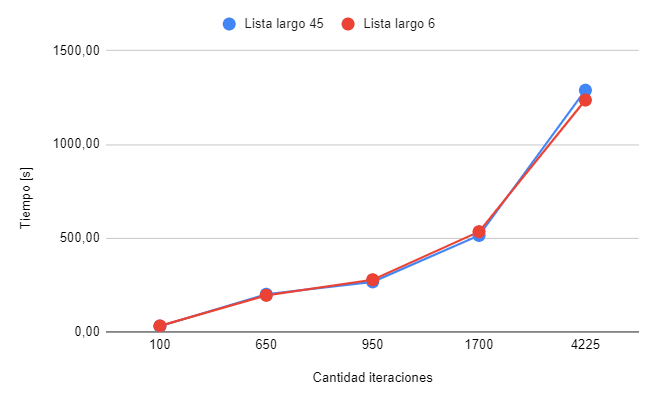
\includegraphics[width=\textwidth]{iter_time.png}
\end{figure}
Con respecto a los tiempos se puede apreciar que, al aumentar la cantidad de iteraciones, aumenta el tiempo de cómputo, pero no necesariamente aumenta drásticamente el tiempo debido a la variación del tamaño de la lista.

\newpage
Para el experimento de variar el largo de la lista, dónde se consideran 1700 iteraciones como valor fijo, se obtienen los siguientes resultados.

\begin{table}[ht]
\centering
\begin{tabular}{|c|c|c|}
\hline
\multicolumn{1}{|l|}{Iteración} & \multicolumn{1}{l|}{Tiempo {[}s{]}} & \multicolumn{1}{l|}{calidad} \\ \hline
6   & 561,95 & 39 \\ \hline
47  & 555,31 & 30 \\ \hline
72  & 549,91 & 28 \\ \hline
564 & 451,20 & 21 \\ \hline
\end{tabular}
\caption{Resultados tiempo/calidad de las variaciones de la lista tabú para 1700 iteraciones.}
\label{table:tf}
\end{table}
Se puede notar que a menor tamaño de la lista existe una mayor calidad de la solución, y que al intentar diversificar con una lista de mayor tamaño, la calidad va solo en descenso, probablemente la topología del espacio de soluciones candidatas es un ``\textit{gran montículo}", dónde solo va en descenso, en cuanto al tiempo se puede apreciar que a mayor tamaño de la lista, menos tiempo se demora, dado que el algoritmo está diseñado para saltar las soluciones candidatas prohibidas.

\section{Conclusiones}
\subsection{Trabajo interno}
    Se puede notar que la solución final es entregada por \textit{Greedy} y luego Tabu search con cualquier variación de parámetros no llega a una solución mejor que las 45 unidades de calidad entregada por el primero, por lo que podemos suponer que \textit{Greedy} encuentra el óptimo local y luego \textit{Tabu Search} no logra escapar de este haciendo solo descenso. Existe la posibilidad de que en la primera parte se encuentre la única mejor solución debido a que los pacientes en un principio fueron asignados lo más antes posible (razón por la que se estudian las ``preferencias"), y además se asignan los primeros doctores/máquinas disponibles, siendo todos situados en el mismo orden al momento de encolar, por lo que \textit{greedy} para esta instancia en particular, obtiene los mejores resultados.
    Por otra parte considerando las mejores soluciones entregadas por \textit{Tabu Search} se puede apreciar que al acortar el tamaño de la cola, la calidad es mayor, puesto que se parte en un máximo y luego al intentar escapar del óptimo local diversificando, se aceptan soluciones de peor calidad, pero para los casos estudiados, nunca se vuelve a encontrar otro óptimo por el cuál escalar y mejorar la mejor solución.
\subsection{Trabajo externo}
Se puede notar que el problema presentado de agendar pacientes a radioterapia es un problema ampliamente abordado, que tiene distintas instancias o enfoques, dado que se puede considerar las preferencias de pacientes o su llegada por teoría de colas\cite{cartoce}, también si no se consideran los doctores en el problema, o si que las máquinas sean distintas por su consumo de energía\cite{siete}. Las técnicas con mejores resultados en la literatura tienen en común ser '\textit{online algorithms}', es decir, los pacientes se programan uno a uno en tiempo real.

Dentro de las soluciones más prometedoras está SFOM, basado en la idea de aprovechar el patrón ASAP y de preasignar diferentes turnos a pacientes de diferentes categorías. que además bajo su estudio es capaz de tratar a todos los pacientes urgentes y la mayoría de los pertenecientes a las otras categorías.

\subsection{Trabajo futuro}

Los trabajos a futuro para realizar son considerando las preferencias del paciente y el factor degenerativo que tienen, y por ende aumentan el tiempo que necesitan estar en tratamiento utilizando una máquina. Se podría investigar el uso de algoritmos look-head para analizar el rendimiento del modelado\cite{trece}, también se podría 'internacionalizar' el modelo, dado que los supuestos y restricciones se deben ajustar al modelo de salud de cada país.

Además, se debería investigar el comportamiento de tabú search pero para instancias con más restricciones, como por ejemplo que se considere un lista de pacientes en espera, los cuales correspondan a nuevos pacientes, o a los que quedaron pendientes de la calendarización anterior. Por otro lado, se debería analizar el suavizar restricciones, como el inicio de un tratamiento para un paciente, esto enfocado para aquellos días en el calendario que quedan sin atender a ningún paciente, esto debido a que hay pacientes que aún no pueden ser atendidos por restricción. En cuanto a las mejoras de este algoritmo se tiene que \textit{Greedy} construye rápidamente una solución factible, y además bastante buena para las restricciones de este trabajo, a pesar de que la lista tabú no logra obtener mejores resultados, no se debería descartar como algoritmo para facilitar soluciones, más bien se debería hacer un estudio más a profundidad, con otro tipo de restricciones, como se menciona anteriormente. 



\bibliographystyle{unsrt}
\bibliography{Referencias}

\end{document}